\documentclass[a4paper,10pt]{article}
\usepackage[utf8]{inputenc}
\usepackage{graphicx}
\usepackage{listingsutf8}
\usepackage{xcolor}
\usepackage{float}

%%%%%%%%%%%%%%%%%%%%%%%%%%%%%%%%%%%%%%%
\lstnewenvironment{algo}[1][]
{
  \lstset{ % c'est le style
    frame=tB,
    numbers=left,
    numberstyle=\tiny,
    basicstyle=\ttfamily\small,
    identifierstyle=\color{black}\bfseries,
    keywordstyle=\color{LightSeaGreen}\bfseries,
    keywords={ALGORITHME, PROGRAMME, ALGO, VAR, DONNEES, VARIABLES,
      DEBUT, FIN, SI, ALORS, FSI, SINON, ET, OU, NON, TQ, FTQ, FAIRE,
      POUR, FPOUR, ALLOUER, RENVOYER},
    numbers=left,
    stepnumber=1,
    xleftmargin=.04\textwidth
  }
}
{}

%%%

\title{Rapport I53 - Projet de fin de semestre\\Conception d'un compilateur ALGO / RAM}
\author{SWAILEM Abdullah – BA GUBAIR Emad}
\date{28/12/2023}

\begin{document}
\maketitle

\section*{Introduction}
\begin{itemize}
    \item Nous avons réussi à compiler le programme contenu dans le fichier \texttt{example12.algo}, dans lequel nous indiquons ce qui ne fonctionne pas encore.
    \item Dans le répertoire test, il y a des exemples numérotés de 1 à 12.
    \item Pour faciliter l'exécution du code, nous récupérons le code de la machine RAM de M. Zanotti. Ensuite, pour compiler notre algorithme, nous utilisons la commande :
    \begin{itemize}
        \item \texttt{/bin/arc "./test/exemple\{file\_number\}.algo"}
    \end{itemize}



    \item Vous pouvez l'exécuter avec la commande :
        \begin{itemize}
            \item  \texttt{node ./ram/ram.js out.ram ./ram/input}
        \end{itemize}
    \item Dans le fichier "input", nous mettons les valeurs des données d'entrée.

    \item Pour faciliter les tests de code, vous pouvez utiliser la commande :
    \begin{itemize}
        \item \texttt{./test -\{option\} file\_number}
    \end{itemize}

\item Les options sont les suivantes :

    \begin{itemize}
       \item "-l"  lire
       \item  "-c"  compiler
       \item "-e"  compiler et exécuter
       \item "-h"  liste de example

    \end{itemize}
\item

\item Dans les sections suivantes, nous expliquerons en détail chaque fichier individuel du projet.
\end{itemize}
\subsection*{Analyse lexicale (\texttt{lexer.lex}) - Reconnaissance du vocabulaire}
Il s'agit du découpage du flot de données en unités lexicales, en accord avec le code portant du sens. pour l'exemple 6:

\begin{algo}
VAR g<-9
PROGRAMME()
VAR taille,t[5], @p
DEBUT
    ALLOUER( p, 10 )
    taille <- 5+3
    t[0] <- 1
    p[0] <- 5
FIN
\end{algo}





\begin{itemize}
 \item \texttt{<PROGRAMME, "PROGRAMME">}
 \item \texttt{<(, "(">}
 \item \texttt{<), ")"> }
 \item \texttt{<VAR, "VAR">}

 \item ..
\end{itemize}

\subsection*{Analyse syntaxique (\texttt{parser.y, asa.h, asa.c})}
Il prend les unités lexicales et produit une structure reflétant la grammaire du langage.

\subsection*{Affichage avec DOT}
Pour faciliter la visualisation et la gestion de la structure arborescente de notre programme, nous avons utilisé l'outil DOT. Cette technique s'est avérée être une solution claire et intuitive pour représenter l'arbre syntaxique généré par le compilateur. Pour le dernier exemple, l'image ci-dessous représente cette structure .

\begin{figure}[H]
    \centering
    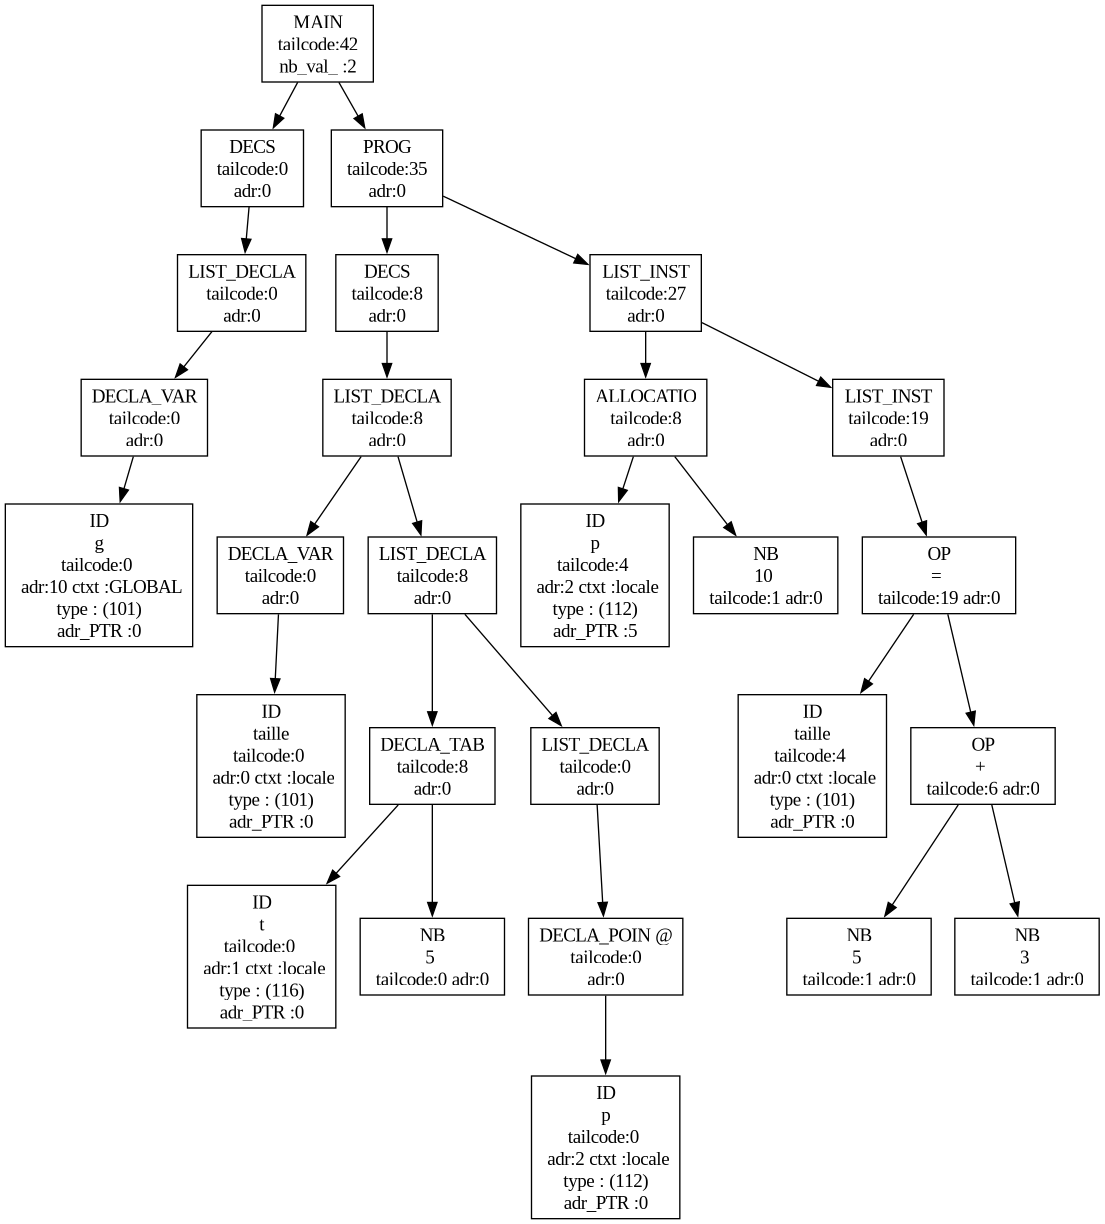
\includegraphics[width=0.8\textwidth]{asa.png}
    \caption{Arbre syntaxique généré par le compilateur pour example 6}
    \label{fig:asa_structure}
\end{figure}

\subsection*{Analyse sémantique (\texttt{Semantic.c, ts.c})}
Elle utilise l'arbre abstrait pour vérifier le sens des instructions.

\begin{itemize}
    \item Elle permet de détecter les erreurs:
    \begin{enumerate}
        \item Mauvais typage
        \item Incompatibilité de type
        \item Déclaration de variables et ajout dans la table des symboles
        \item Dépassement de mémoire
    \end{enumerate}
    \item Nous avons ajouté une fonction : \texttt{int error\_semantic(const char *s)} pour gérer les erreurs sémantiques.
    \item Les fonctions \texttt{semantic\_decla\_..} gèrent la déclaration de variables, qu'elles soient locales ou globales.
    \begin{enumerate}
        \item Pour chaque déclaration  nous vérifions s'il a déjà été déclaré, que ce soit dans la portée globale ou locale. Si oui, une erreur est affichée.
        \item Pour chaque appel  nous vérifions s'il a déjà été déclaré, que ce soit dans la portée globale ou locale. Si non , une erreur est affichée.
        \item Les variables globales vont dans le segment de données, tandis que les variables locales vont dans la pile
        \item \texttt{INT "VAR x" :} Toutes les variables doivent être déclarées et avoir une adresse avant leur premier usage, et elles ne peuvent pas être redéclarées .
        \item  \texttt{TAB " VAR T[5] :}
       \item \texttt{PTR "VAR @P" : } \texttt{ALLOUER(P,5) } pour allocation dynamique
            \begin{enumerate}
                \item La taille doit être un nombre entier (pas d'expressions, même constantes)
                \item Ils ont leur adresse dans la pile où ils stockent leur première adresse vers le tas.
                \item Vous pouvez récupérer leur valeur par \texttt{P[5], T[i]}.
            \end{enumerate}


    \end{enumerate}
     \item \texttt {Fonctions} :Quand on déclare une fonction, on réserve l'espace mémoire pour ses paramètres, ses variables locales de contexte \texttt {"nom de fonction"}, et on stocke l'adresse de la première instruction de la fonction dans l'adresse de fonction dans le segment de données. Pour l'appeler, nous commencerons par remplacer les valeurs des variables\texttt {"par valeur"} ou leur adresse\texttt {"par adresse"} .

            \begin{algo}
            //définies comme suit :
            ALGO ID( L_param )
            DEBUT
                //L_inst
            FIN

            \end{algo}
    \item Le variable  \texttt{int VLOCAL} : pour numéroter les variables locales, commençant par 0. Le nombre présent représente son adresse dans la pile et est ajouté à la table des symboles.
    \item Le variable  \texttt{int VGLOBAL } : : pour numéroter l'adresse de la variable globale, commençant par le début du segment donné. Son adresse est directement présentée dans la RAM.
    \item Le variable  \texttt{int ADRPTR} :  Nous attribuons le premier pointeur qui pointera vers le tas à l'adresse 0. Cela signifie qu'il prendra la première adresse dans le tas, et ensuite nous attribuerons la suivante en ajoutant la taille du premier. Par exemple, si nous déclarons au début un pointeur de taille 5, il prendra les adresses de 0 à 4, et ensuite le suivant commencera à 5.
    \item Table des symboles pour gérer les identificateurs comme dans l'image suivante  :
\end{itemize}
\begin{figure}[H]
    \centering
    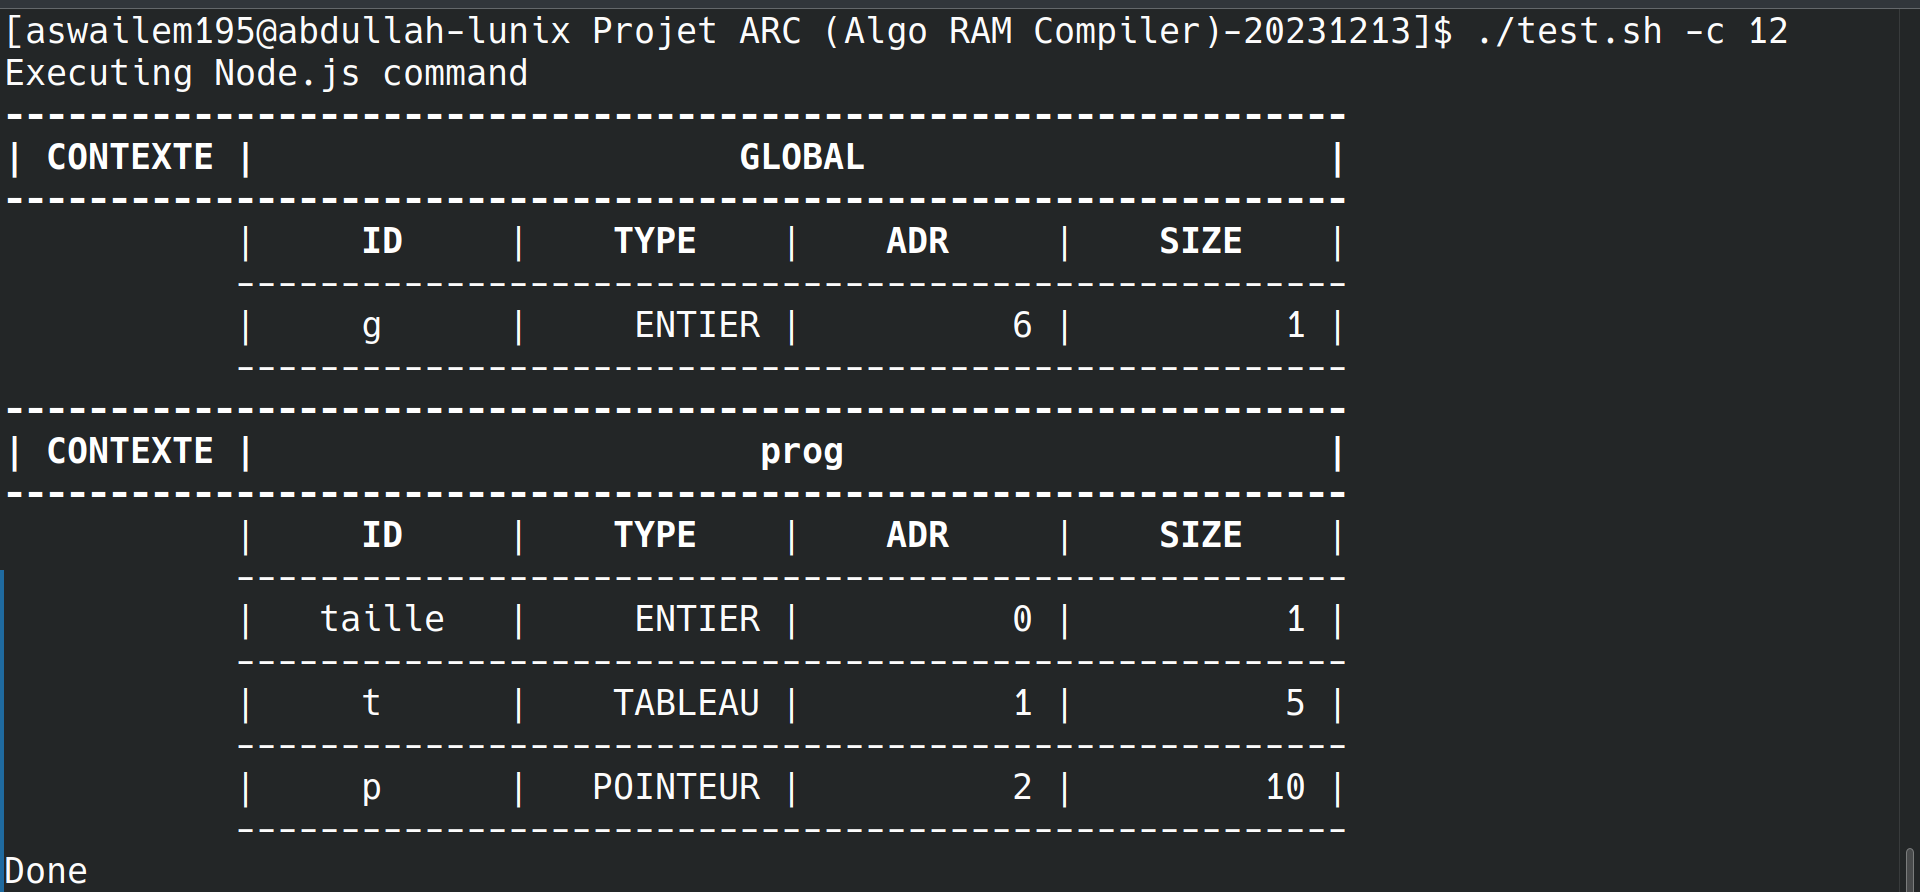
\includegraphics[width=0.8\textwidth]{ts.png}
    \caption{Table des symboles example 6 }
    \label{fig:asa_structure}
\end{figure}

\subsection*{Génération de code intermédiaire}
\begin{itemize}
    \item Génère du code pour une machine RAM.
    \item La structure de la mémoire:
    \begin{itemize}
        \item Registre 0: ACC
        \item Registre 1: \texttt{RAM\_OS\_TMP\_REG 1 //registre temporaire}
        \item Registre 2: \texttt{RAM\_OS\_STK\_REG 2 //le début de pile}
        \item Registre 3: \texttt{RAM\_OS\_ADR\_REG 3 //sommet de pile}
        \item Registre 4: \texttt{RAM\_OS\_TAS\_REG 4 // début de tas}
        \item Registre 5: \texttt{RAM\_OS\_EMPILER\_ADR 5 //pour le moment je l'utilise pour l'appel et le retour de fonction}
        \item Registre 6: \texttt{VGLOBAL = 6 // Pour numéroter l'adresse de la variable globale, on utilise int dans semantic.c.}
        \item \texttt{PILE\_DEBUT\_ADR 32}
        \item \texttt{TAS\_DEBUT\_ADR 150}
    \end{itemize}
    \item Nous considérons que la portée des variables locales reste restreinte à toute la vie du code, mais on ne peut pas les utiliser juste dans leur fonction gérée par le \texttt{semantic.c}.
    \item En ce qui concerne le tas, je lui donne une adresse, mais toujours, on insère à l'adresse avant. Cela pourrait dire que son adresse est décroissante.
    \item L'image suivante présente la structure de la mémoire pour l'exemple 6 :
\begin{figure}[H]
    \centering
    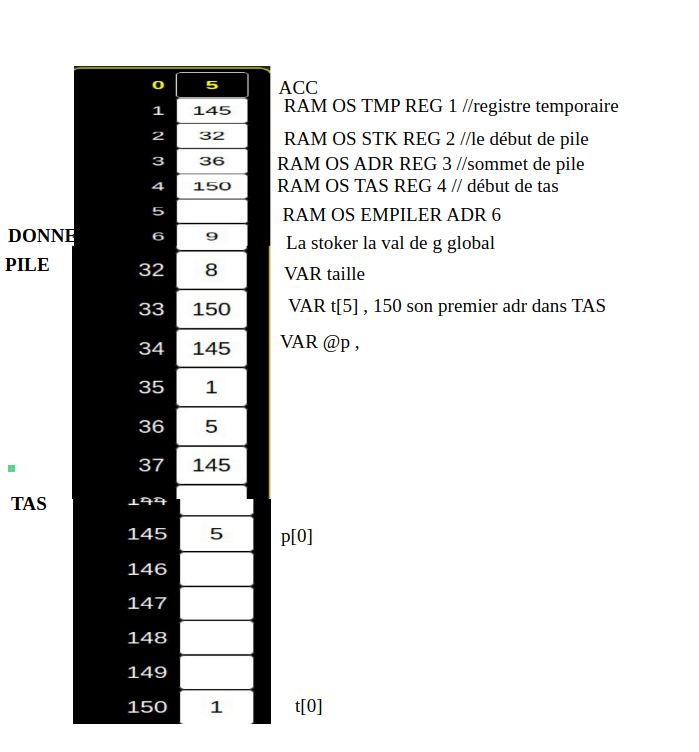
\includegraphics[width=0.8\textwidth]{RAM.png}
    \caption{structure de RAM example 6}
    \label{fig:asa_structure}
\end{figure}
\end{itemize}

\end{document}
